%
%===============>>  ПРОБНИК 1 <<=============
%
%BEGIN_FOLD % ====>>_____ Вариант 1 _____<<====
\begin{training}[1]
	\begin{listofex}
	\item Больному прописано лекарство, которое нужно пить по \(0,5\) г \(3\) раза в день в течение \(21\) дня. В одной упаковке \(10\) таблеток лекарства по \(0,5\) г. Какого наименьшего количества упаковок хватит на весь курс лечения?
	%2
	\item Установите соответствие между величинами и их возможными значениями: к каждому элементу первого столбца подберите соответствующий элемент из второго столбца. \\
	\begin{minipage}[t]{0.58\linewidth}
		\textbf{Величины:}
		\begin{tasks}
			\task площадь одной страницы учебника
			\task площадь территории республики Карелия
			\task площадь одной стороны монеты
			\task площадь бадминтонной площадки
		\end{tasks}
	\end{minipage}
	\hspace{0.05\linewidth}
	\begin{minipage}[t]{\textwidth}
		\textbf{Возможные значения:}
		\begin{tasks}
			\task \(81,7\) кв. м
			\task \(330\) кв. см
			\task \(180,5\) тыс. кв. км
			\task \(300\) кв. мм
		\end{tasks}
	\end{minipage}
	%3
	\item На диаграмме показана среднемесячная температура в Нижнем Новгороде (Горьком) за каждый месяц \(1994\) года. По горизонтали указываются месяцы, по вертикали --- температура в градусах Цельсия. Определите по диаграмме наименьшую среднемесячную температуру в \(1994\) году. Ответ дайте в градусах Цельсия
	\begin{minipage}[t]{\linewidth}
		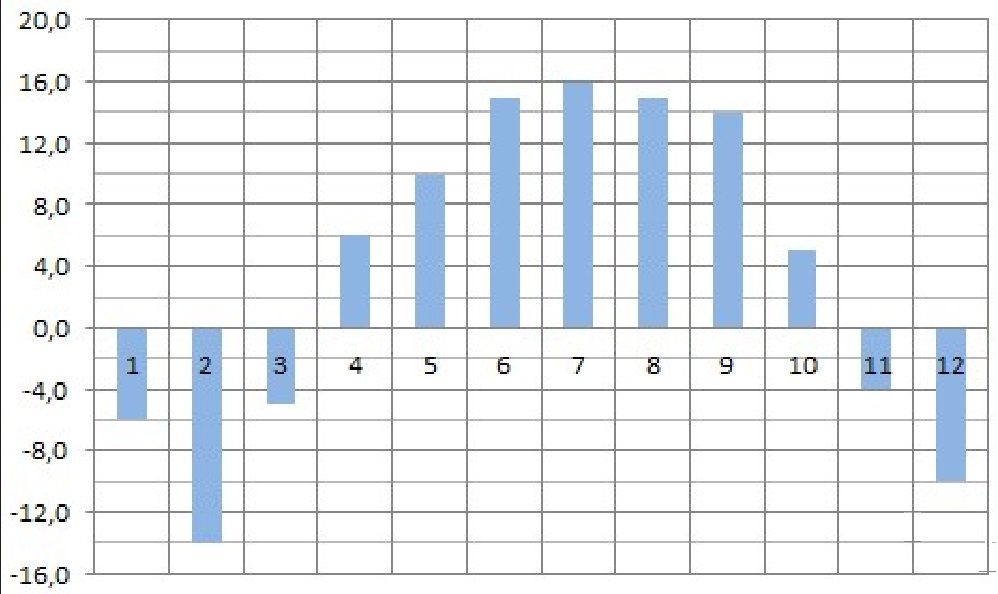
\includegraphics[align=t, width=\linewidth]{../pics/G101M8H3-3}
	\end{minipage}
	\item В фирме «Эх, прокачу!» стоимость поездки на такси (в рублях) рассчитывается по формуле \(C=150+11\cdot (t-5)\), где \(t\) --- длительность поездки, выраженная в минутах \((t>5)\). Пользуясь этой формулой, рассчитайте стоимость \(8\)-минутной поездки.
	\item Перед началом футбольного матча судья бросает монетку, чтобы определить, какая из команд начнёт игру с мячом. Команда «Физик» играет три матча с разными командами. Найдите вероятность того, что в этих играх «Физик» выиграет жребий ровно два раза.
	%6
	\item 
	\begin{minipage}[t]{\linewidth}
		Для изготовления книжных полок требуется заказать \(48\) одинаковых стекол в одной из трех фирм. Площадь каждого стекла \(0,25\) м\(^2\). В таблице приведены цены на стекло, а также на резку стекол и шлифовку края. Сколько рублей будет стоить самый дешевый заказ?
	\end{minipage}
	\hspace{0.02\linewidth}
	\begin{minipage}[t]{\linewidth}
		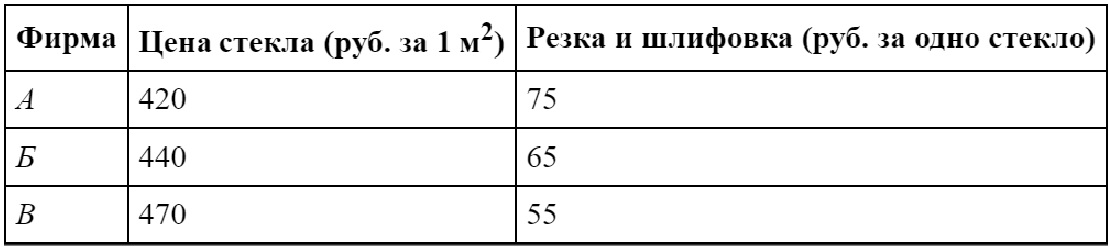
\includegraphics[align=t, width=\linewidth]{../pics/G101M8H3-6}
	\end{minipage}
	%7
	\item 
	\begin{minipage}[t]{\linewidth}
		Установите соответствие между графиками линейных функций и угловыми коэффициентами прямых.
	\end{minipage}
	\hspace{0.02\linewidth}
	\\
	\textbf{Графики:}
	\\
	\begin{minipage}[t]{\linewidth}
		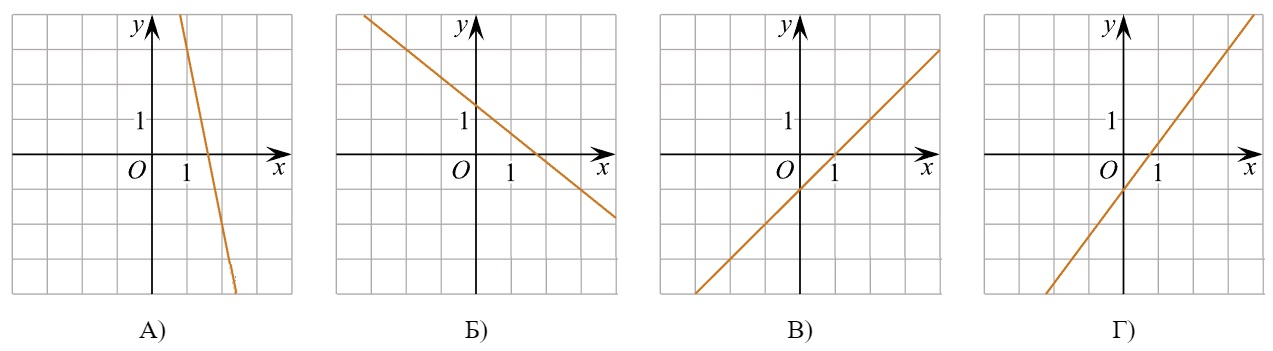
\includegraphics[align=t, width=\linewidth]{../pics/G101M8L6-3}
	\end{minipage}
	\\
	\\
	\textbf{Угловые коэффициенты:}
	\begin{tasks}(4)
		\task \( \dfrac{ 4 }{ 3 } \)
		\task \( -5 \)
		\task \( -0,8 \)
		\task \( 1 \)
	\end{tasks}
	\item Средний балл выпускника школы, сдавшего ЕГЭ по четырём предметам, составляет \(75\). Самый низкий результат он показал по математике --- \(66\) баллов (по остальным экзаменам баллы выше). Выберите утверждения, которые следуют из приведённых данных.
	\begin{tasks}
		\task Средний балл по трём экзаменам, кроме математики, равен \(78\)
		\task Минимальный балл по любому из трёх предметов, не считая математики, больше \(75\)
		\task Ни по одному предмету выпускник не получил \(100\) баллов
		\task По какому-то предмету выпускник получил больше \(76\) баллов
	\end{tasks}
	%9
	\item
	\begin{minipage}[t]{0.68\linewidth}
		Найдите площадь четырехугольника, изображенного на клетчатой бумаге с размером клетки \(1\) см на \(1\) см (см. рис.). Ответ дайте в квадратных сантиметрах.
	\end{minipage}
	\hspace{0.02\linewidth}
	\begin{minipage}[t]{0.27\linewidth}
		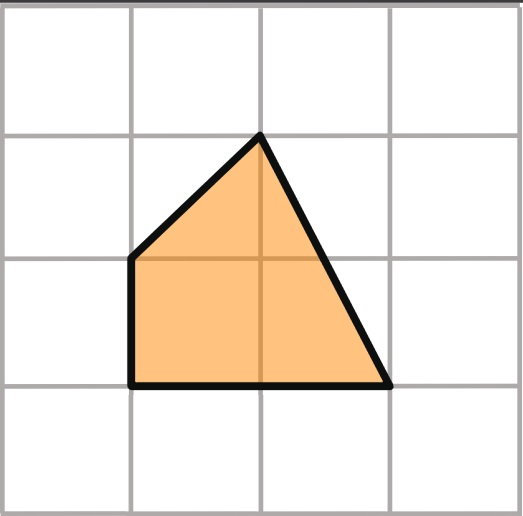
\includegraphics[align=t, width=\linewidth]{../pics/G101M8H3-9}
	\end{minipage}
	%10
	\item
	\begin{minipage}[t]{0.68\linewidth}
		Дачный участок имеет форму прямоугольника со сторонами \(20\) метров и \(30\) метров. Хозяин планирует обнести его забором и разделить таким же забором на две части, одна из которых имеет форму квадрата. Найдите общую длину забора в метрах.
	\end{minipage}
	\hspace{0.02\linewidth}
	\begin{minipage}[t]{0.27\linewidth}
		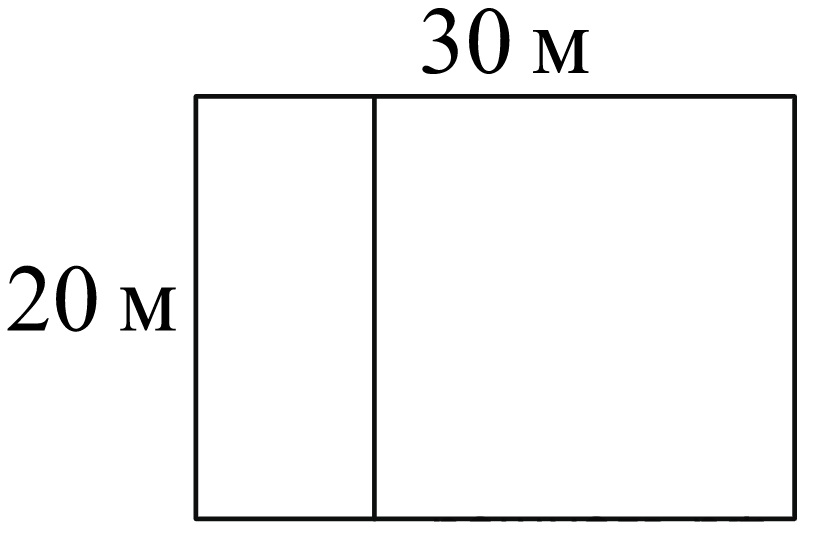
\includegraphics[align=t, width=\linewidth]{../pics/G101M8H3-10}
	\end{minipage}
	%11
	\item
	\begin{minipage}[t]{0.68\linewidth}
		В бак, имеющий форму прямой призмы, налито \(12\) л воды. После полного погружения в воду детали, уровень воды в баке поднялся в \(1,5\) раза. Найдите объём детали. Ответ дайте в кубических сантиметрах, зная, что в одном литре \(1000\) кубических сантиметров.
	\end{minipage}
	\hspace{0.02\linewidth}
	\begin{minipage}[t]{0.27\linewidth}
		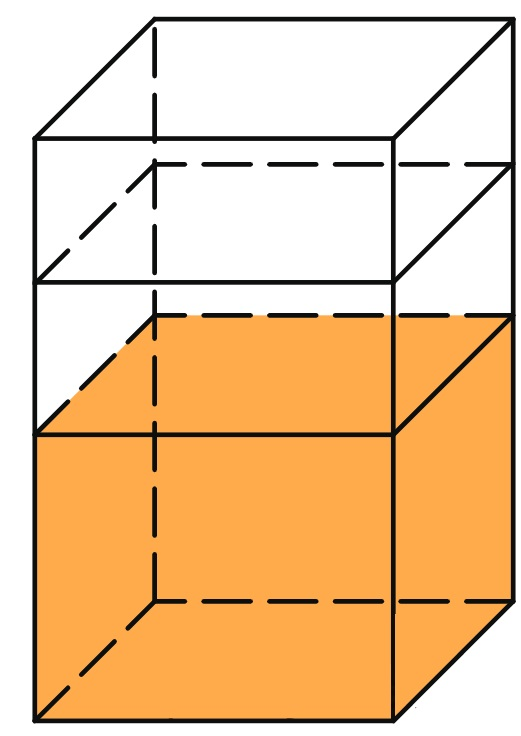
\includegraphics[align=t, width=\linewidth]{../pics/G101M8H3-11}
	\end{minipage}
	\item Катеты прямоугольного треугольника равны \(6\) и \(8\). Найдите наибольшую среднюю линию треугольника.
	\item Два ребра прямоугольного параллелепипеда равны \(7\) и \(4\), а объём параллелепипеда равен \(140\). Найдите площадь поверхности этого параллелепипеда.
	\item Найдите значение выражения: \(\dfrac{ 14 }{15  }:\dfrac{ 7 }{ 3 }-0,5\)
	\item Только \(94\%\) из \(27 500\) выпускников города правильно решили задачу \(B1\). Сколько человек правильно решили задачу \(B1\)?
	\item Найдите значение выражения: \(\dfrac{ 4^{3,5}\cdot 5^{2,5} }{ 20^{1,5} }\).
	\item Найдите корень уравнения: \( \sqrt{13+2x}=5 \)
	%18
	\item Каждому из четырёх чисел в левом столбце соответствует отрезок, которому оно принадлежит. Установите соответствие между числами и отрезками из правого столбца. \\
	\begin{minipage}[t]{0.55\linewidth}
		\textbf{Числа:}
		\begin{tasks}
			\task \( \log_210 \)
			\task \( \dfrac{7}{3} \)
			\task \( \sqrt{26} \)
			\task \( 0,6^{-1} \)
		\end{tasks}
	\end{minipage}
	\hspace{0.02\linewidth}
	\begin{minipage}[t]{0.4\linewidth}
		\textbf{Решения:}
		\begin{tasks}
			\task \( [1;2] \)
			\task \( [2;3] \)
			\task \( [3;4] \)
			\task \( [5;6] \)
		\end{tasks}
	\end{minipage}
	\item Цифры четырёхзначного числа, кратного \(5\), записали в обратном порядке и получили второе четырёхзначное число. Затем из первого числа вычли второе и получили \(1458\). Приведите ровно один пример такого числа.
	\item Теплоход проходит по течению реки до пункта назначения \( 513 \) км и после стоянки возвращается в пункт отправления. Найдите скорость теплохода в неподвижной воде, если скорость течения равна \( 4 \) км/ч, стоянка длится \( 8 \) часов, а в пункт отправления теплоход возвращается через \( 54 \) часа после отплытия из него. Ответ дайте в км/ч.
	\item В доме всего \(14\) квартир с номерами от \(1\) до \(14\). В каждой квартире живёт не менее \(1\) и не более \(4\) человек. В квартирах с \(1\)-й по \(12\)-ю включительно живёт суммарно \(14\) человек, а в квартирах с \(11\)-й по \(14\)-ю включительно живёт суммарно \(12\) человек. Сколько всего человек живут в этом доме?
	\end{listofex}
\end{training}
%END_FOLD